With the complete graph $K_4$, we will illustrate our construction,
its evaluation and an interpretation
in terms $K_4$'s familiar linear spaces, oriented matroids, and electrical
network problem model.  $P=\{p_1, p_2\}$ is comprised of two non-adjacent
edges and the rest, $K_{2,2}$, will comprise $E$.  

We relate $K_4$ as a 1-dimensional abstract simplicial complex to
its role as an electrical network model.
To make cycles represent flows of positive current,
coboundaries electrical potentials and resistance positive,
our sign conventions for arbitrarilly oriented labeled (multi)graphs
will be \emph{opposite that of} the homology of 1-dimensional chain complexes:
For $e : a \rightarrow b$, $\partial_1(e)=a-b$, $\partial^0(\hat{a})=\hat{e}+ \ldots\  $,
$\partial^0(\hat{b})=-\hat{e}+ \ldots\  $, where $e$ is edge with end vertices $a$ and $b$ oriented
as indicated\
\footnote{
On the other hand, for the sake of mathematical simplicity,
we will use this sign convention the port edges (in $P$).
In electrical engineering
circuit theory writings the sign convention for ports is reversed
so quantities characterizing typical system behavior
observable at the ports
are positive.}.
With $\partial^0(\phi(\hat{a}) \hat{a} + \phi(\hat{b}) \hat{b}) = (\phi(\hat{a})-\phi(\hat{b}))\hat{e} + \cdots$,
$\phi(\hat{a})-\phi(\hat{b})$ is the voltage drop going from $a$ to $b$.
Edge sets $E$ and $P$ will respectively represent resistors and ports.
When $e\in E$,
Ohm's law says that
the voltage drop  $\phi(\hat{a})-\phi(\hat{b})$ across $e$ is the
resistance of $e$ 
times the current through $e$,
flowing from $a$ to $b$.
For us, the currents through and voltage drops along
in all these edges are variables $i_t$ and $v_t$ for $t\in P\cup E$.  Ohm's law
is asserted in the homogeneous form\cite{SmithElec,TutteEx,CirThProjHomo2019}:  For $e\in E$, the voltage-drop-to-current ratio
$v_e:i_e$ $=$ $r_e:g_e$, the ratio of the resistivity parameters.
Those parameters are not given for ports.
Kirchhoff's voltage law asserts that $\sum_tv_t\hat{t}$ is the 1-coboundry $\partial^0(\sum \phi(\hat{a})\hat{a})$
for some $\phi:V\rightarrow K$; physically, $\phi$ is the electrical potential function.
Kirchhoff's current law asserts that $\sum_ti_t t$ is a 1-cycle, i.e., in $\text{ker }\partial_1$. 
The problem of linear electrical network analysis is to characterize
the linear relationships among port current and voltage drop variables implied by
the network topology, Kirchhoffs' and Ohm's laws.  


Let $P=\{p_1, p_2\}$ and $E=\{e_1, e_2, e_3, e_4\}$ together be the edges in the (oriented) graph
below representing an electrical network, where $E$ represents the resistors.   $N_\alpha$ is
a full-row-rank, all-column submatrix of the matrix form for $\partial^1$.  It is the
usual signed vertex-edge incidence matrix which represents our graph's graphic matroid, with one
row deleted so $N_\alpha$ has full row rank.  The rows of $N_\alpha$ hold the coefficients in
Kirchhoff's current law, asserting that the edge currents constitute a 1-cycle, (i.e., a flow.)
$N_\beta^\perp$ is a totally unimodular matrix whose
rows are a basis for the 1-cycle space, conveniently
obtainable by coding the incidences of edges with the oriented fundamental
circuits each associated to an edge not in a fixed spanning tree.
Its rows hold the coefficients in
Kirchhoff's voltage law, asserting that the edge
voltages drops constitute a 1-coboundary, differences
of a potential along edges.
This well-known construction gives
two full row rank totally unimodular matrices whose row spaces are orthogonal complements,
representing our graph $G$'s
graphic (with bases $\mathcal{B}(G)$) and cographic matroids respectively.

\begin{figure}
  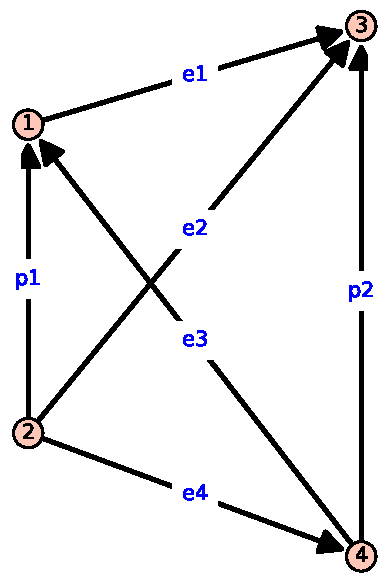
\includegraphics[scale=0.5]{K4.pdf}
\end{figure}

We begin with the familiar incidence matrix representation of $K_4$'s matroid.
We delete row 2 and take a representation for the dual that is consistent
with our exterior algebra duality operator (\ref{dualdefinition}):


\[
\left(\begin{array}{cc|cccc}
1 & 0 & -1 & 0 & 1 & 0 \\
-1 & 0 & 0 & -1 & 0 & -1 \\
0 & 1 & 1 & 1 & 0 & 0 \\
0 & -1 & 0 & 0 & -1 & 1
\end{array}\right)
\;\;\;
N_\alpha=
\left(\begin{array}
{cc|cccc}
1 & 0 & -1 & 0 & 1 & 0 \\
0 & 1 & 1 & 1 & 0 & 0 \\
0 & -1 & 0 & 0 & -1 & 1
\end{array}\right)
%\]
\;\;\;\;
%\[
N_\beta^\perp =
\left(\begin{array}{cc|cccc}
1 & 0 & 0 & 0 & -1 & -1 \\
0 & 1 & 0 & -1 & 0 & 1 \\
0 & 0 & 1 & -1 & 1 & 1
\end{array}\right)
\]


We form the following system of equations according to (\ref{LmatrixDef}).

\begin{equation}\label{K4Equation}
\begin{split}
  0=L\left(\begin{array}{cc} {\Nal} \\ {\NbePe}  \end{array}\right)z
    =& \left[\begin{array}{c|c|c} \Nal(P)  &  0  &  \Nal(E)G \\  \hline
        0  & \NbePe(P)  &  \NbePe(E)R \end{array}\right]
    \left[ \begin{array}{c} i_{p_1} \\ i_{p_2} \\ v_{p_1} \\ v_{p_2} \\ x_{e_1} \\ x_{e_2} \\ x_{e_3} \\ x_{e_4}
      \end{array}
      \right]
    \\
    =&
\left(\begin{array}{cc|cc|cccc}
1 & 0 & 0 & 0 & -g_{1} & 0 & g_{3} & 0 \\
0 & 1 & 0 & 0 & g_{1} & g_{2} & 0 & 0 \\
0 & -1 & 0 & 0 & 0 & 0 & -g_{3} & g_{4} \\ \hline
0 & 0 & 1 & 0 & 0 & 0 & -r_{3} & -r_{4} \\
0 & 0 & 0 & 1 & 0 & -r_{2} & 0 & r_{4} \\
0 & 0 & 0 & 0 & r_{1} & -r_{2} & r_{3} & r_{4}
\end{array}\right)z
\end{split}
\end{equation}


The electrical network problem at hand is to determine linear constraints on the
port variables $i_p, v_p$, $p\in P = \{p_1, p_2\}$ imposed by the system.  In other words,
we want a linear map $M$ on the $K$-vector space with basis $P_\alpha, P_\beta$ whose kernel
is the projection of this system's solution space.
Below is a solution.
We set $r_e=1$ for $e\in E$, and $D=g_{1} g_{2} g_{3} + g_{1} g_{2} g_{4} + g_{1} g_{3} g_{4} + g_{2} g_{3} g_{4}$.
\begin{equation}\label{K4Soln}
M\left(\begin{array}{c} i_{p1} \\ i_{p2} \\ v_{p1} \\ v_{p2}
\end{array}\right) =
\left(\begin{array}{cccc}
{\left(g_{1} + g_{2}\right)} {\left(g_{3} + g_{4}\right)} & -g_{2} g_{3} + g_{1} g_{4} & D & 0 \\
-g_{2} g_{3} + g_{1} g_{4} & {\left(g_{1} + g_{3}\right)} {\left(g_{2} + g_{4}\right)} & 0 & D
\end{array}\right)
\left(\begin{array}{c} i_{p1} \\ i_{p2} \\ v_{p1} \\ v_{p2}
\end{array}\right) = 0
\end{equation}


To compute $\ext{L}_E$ from its definition, set 
$z=[\ext{p}_{\alpha 1},\ext{p}_{\alpha 2},\ext{p}_{\beta 1},\ext{p}_{\beta 2},
  \ext{e}_1,  \ext{e}_2,  \ext{e}_3,  \ext{e}_4]^t$
in the right hand side of (\ref{K4Equation}) 
and expand in terms of this basis
the exterior product (in order) of the resulting column's entries.
Finally, we select
the terms that can be expressed as
$\ext{T}\ext{e}_1\ext{e}_2\ext{e}_3\ext{e}_4$.
The final
value is the sum of such $\ext{T}$; it is a $K$-multiple of exterior
row product of $M$, i.e., $M_1\ext{z}\wedge M_2\ext{z}$ where
$\ext{z}$ $=$ 
$[\ext{p}_{\alpha 1},\ext{p}_{\alpha 2},\ext{p}_{\beta 1},\ext{p}_{\beta 2}]^t$.
Each $\ext{T}$ is the $\wedge$ of unique pair of distinct elements
of $\{\ext{p}_{\alpha 1}, \ext{p}_{\alpha 2}, \ext{p}_{\beta 1}, \ext{p}_{\beta 2}\}$
with a coefficient that is a polynomial in the 
$g_e$, $r_e$.  These coefficients are \Plucker coordinates
for the orthogonal complement of the electrical network's
(itself parametrized by the $g_e, r_e$) solution space.
Each polynomial
term encodes a subset of $E=\{e_1, e_2, e_3, e_4\}$, for example, $\{e_1, e_2\}$ is encoded
by $g_1g_2r_3r_4$. Note that each coefficient enumerates
the common bases of a pair of not always distinct matroid minors.  See \ref{commonbasescoro}.


\begin{equation}\label{K4table}
\begin{array}{|c|c|c|} \hline
\text{basis element} & \text{coefficient} & \text{enumerates bases}\\
  \hline

\ext{p}_{\alpha 1}\ext{p}_{\alpha 2} &
g_1 + g_2 + g_3 + g_4 & \mathcal{B}(G/\{p_1, p_2\})

\\ \hline

\ext{p}_{\alpha 1}\ext{p}_{\beta 1} &
g_2g_3 - g_1g_4 &  \mathcal{B}(G/p_1\setminus p_2)\cap\mathcal{B}(G/p_2\setminus p_1)

\\ \hline

\ext{p}_{\alpha 1}\ext{p}_{\beta 2} &
(g_1 + g_2)(g_3 + g_4) & \mathcal{B}(G/p_1\setminus p_2)
\\ \hline 

\ext{p}_{\alpha 2}\ext{p}_{\beta 1} & -(g_1 + g_3)(g_2+g_4) & \mathcal{B}(G/p_2\setminus p_1)
\\ \hline
 
\ext{p}_{\alpha 2}\ext{p}_{\beta 2} &
-g_2g_3 + g_1g_4 & \mathcal{B}(G/p_1\setminus p_2)\cap\mathcal{B}(G/p_2\setminus p_1)
\\ \hline
 
\ext{p}_{\beta 1}\ext{p}_{\beta 2} &
g_1g_2g_3 + g_1g_2g_4 + g_1g_3g_4 + g_2g_3g_4 & \mathcal{B}(G\setminus \{p_1, p_2\})
\\ \hline

\end{array}
\end{equation}

To verify that the coefficients of our $\ext{L}_E$
in (\ref{K4table}) are \Plucker coordinates, and
indeed that $\ext{L}_E$ represents the space of
linear constraints for the
network solution problem,
one can calculate that each $2\times 2$ minor of $M$ in
(\ref{K4Soln}) equals the $D$ multiple of the corresponding coefficient
in  (\ref{K4table}).  The one non-trivial calculation is
\[
{\left(g_{1} + g_{2}\right)} {\left(g_{1} + g_{3}\right)} {\left(g_{2} + g_{4}\right)} {\left(g_{3} + g_{4}\right)} - {\left(-g_{2} g_{3} + g_{1} g_{4}\right)}^{2} = D(g_1+g_2+g_3+g_4)
\]

This example also demonstrates that $\ext{L}_E$ might not have a
matrix representation all of whose entries are $K_0$ polynomials in the $r_e, g_e$.

\subsection{Example with $\ext{N}_\alpha\neq\ext{N}_\beta$}
We take $N_\alpha$ from before, but form $N_\beta$ from $N_\alpha$ by replacing $-1$s by $0$.
$N_\beta$ now represents the partition matroid $\Pi$ where
the edges are partitioned according to which vertex
in $\{1, 3, 4 \}$ is its head.


\[
N_\alpha=
\left(\begin{array}
{cc|cccc}
1 & 0 & -1 & 0 & 1 & 0 \\
0 & 1 & 1 & 1 & 0 & 0 \\
0 & -1 & 0 & 0 & -1 & 1
\end{array}\right)
%\]
\;\;\;\;
%\[
N_\beta=
\left(\begin{array}
{cc|cccc}
1 & 0 & 0 & 0 & 1 & 0 \\
0 & 1 & 1 & 1 & 0 & 0 \\
0 & 0 & 0 & 0 & 0 & 1
\end{array}\right)
\;\;\;
N_\beta^\perp =
\left(\begin{array}{cc|cccc}
1 & 0 & 0 & 0 & -1 & 0 \\
0 & 1 & 0 & -1 & 0 & 0 \\
0 & 0 & 1 & -1 & 0 & 0
\end{array}\right)
\]


\begin{equation}\label{K4Dirtable}
\begin{array}{|c|c|c|} \hline
\text{basis element} & \text{coefficient} & \text{enumerates bases}\\
  \hline

\ext{p}_{\alpha 1}\ext{p}_{\alpha 2} &
 g_{4} & \mathcal{B}(G/\{p_1, p_2\}) \cap  \mathcal{B}(\Pi/\{p_1, p_2\})

\\ \hline

\ext{p}_{\alpha 1}\ext{p}_{\beta 1} &
0 &  \mathcal{B}(G/p_1\setminus p_2)\cap\mathcal{B}(\Pi/p_2\setminus p_1)

\\ \hline

\ext{p}_{\alpha 1}\ext{p}_{\beta 2} &
 (g_{1} +  g_{2}) g_{4} & \mathcal{B}(G/p_1\setminus p_2)  \cap \mathcal{B}(\Pi/p_1\setminus p_2)
\\ \hline 

\ext{p}_{\alpha 2}\ext{p}_{\beta 1} &
- g_{3} g_{4} & \mathcal{B}(G/p_2\setminus p_1) \cap \mathcal{B}(\Pi/p_2\setminus p_1)
\\ \hline
 
\ext{p}_{\alpha 2}\ext{p}_{\beta 2} &
 g_{1} g_{4} & \mathcal{B}(G/p_2\setminus p_1)\cap\mathcal{B}(\Pi/p_1\setminus p_2)
\\ \hline
 
\ext{p}_{\beta 1}\ext{p}_{\beta 2} &
 (g_{1} +g_{2}) g_{3} g_{4} & \mathcal{B}(G\setminus \{p_1, p_2\})  \cap \mathcal{B}(\Pi\setminus \{p_1, p_2\})
\\ \hline

\end{array}
\end{equation}



